\chapter{舰基无人机立体视觉引导系统}
\section{引言}
由于视觉传感器具有成本较低和感知信息量较大的特性,该类型传感器被广泛应用于无人机引导与控制领域。本章通过误差分析和理论推导,设计基于立体视觉成像的短基线和长基线引导系统,实现对无人机相对位置的测量。

\section{短基线无人机视觉引导系统}
\subsection{相机成像模型}
本文使用的相机模型为小孔成像模型(Pin-hole Camera Model)。已知目标点$M$的三维空间坐标为$(x,y,z)$,则该坐标与像平面坐标$(u,v)$以及相机焦距$f$之间的关系用其次坐标的形式表达为
\begin{equation}
\lambda\left[ {\begin{array}{*{20}{c}}
	u \\ 
	v \\ 
	f 
	\end{array}} \right] =\left[ {\begin{array}{*{20}{c}}
	x \\ 
	y \\ 
	z 
	\end{array}} \right]
\end{equation}
其中$\lambda$是尺度因子。如果转换为欧拉坐标系,则可以得到
\begin{equation}
\left[ {\begin{array}{*{20}{c}}
	u \\ 
	v 
	\end{array}} \right] =\frac{f}{z} \left[ {\begin{array}{*{20}{c}}
	x \\ 
	y   
	\end{array}} \right]
\end{equation}
则在已知焦距$f$和像平面尺寸$(w_u,w_v)$时,相机水平方向视场角$\alpha_{FOV}$的计算方法为
\begin{equation}
\tan{\frac{\alpha_{FOV}}{2}}=\frac{w_u}{f}
\end{equation}
相机竖直方向视场角$\beta_{FOV}$的计算方法为
\begin{equation}
\tan{\frac{\beta_{FOV}}{2}}=\frac{w_v}{f}
\end{equation}
在求解视场角时,焦距$f$和像平面$(w_u,w_v)$使用的量纲需要统一(像素点或毫米等)。

上述理论模型虽然过于简单,但可以对一些物理量进行初步的估算。已知镜头焦距为$f$,物体的长和高为$W$和$H$,物体到像平面的距离为$L$,物体在像平面的成像尺寸为$w$何$h$,则上述物理量之间的关系为
\begin{align}
f=\frac{wL}{W} \\
f=\frac{hL}{H}
\end{align}
上述公式通常用于对相机镜头选型和理论观测距离的估算。

实际情况中,由于理想光轴不穿过像平面几何中心点、镜头尺寸制作精度等原因,相机的模型一般不符合标准的小孔成像模型,因此需要通过对相机标定(Camera Calibration)的方法,得到内参数和外参数的矩阵表达,从而进一步对像平面上的每个$(u,v)$点进行修正。本文使用ROS中的\texttt{camera\_calibration}\cite{ros_camera_calibration}程序来完成对相机的标定工作。其中最重要的参数是相机的焦距尺寸和主点位置,该程序得到的具体矩阵参数含义可参见文档\cite{ros_camera_message}。

\subsection{传统立体视觉成像原理}
如图\ref{fig:chp03_vision_20_basic_stereo}所示,在光轴平行的情况下,目标$M$在左右两侧像平面的成像的坐标为$(u_l, v_l)$和$(u_r, v_r)$,这里的像平面坐标是经过对标定矩阵对原始坐标修正之后得到的。此时,可以得到目标点与成像坐标之间的关系
\begin{equation}
\left[ {\begin{array}{*{20}{c}}
	x \\ 
	y \\ 
	z 
	\end{array}} \right] =\frac{b}{d} \left[ {\begin{array}{*{20}{c}}
	u_l \\ 
	u_r \\ 
	f 
	\end{array}} \right]
\end{equation}
其中$b$是基线长度,即两个相机之间的距离,$d$是目标在左右相机成像之后的像素值差,即$d=u_l-u_r$。

上述理论模型是基于左右侧相机光轴平行且两个相机焦距相同的情况下的理想立体成像模型,这与实际应用准在偏差,因此需要进一步修正该模型。图\ref{fig:chp03_vision_21_theory_stereo}所示即为两个相机像平面光轴不平行且焦距不同情况。


通过几何关系可以得到以下四个基本公式
\begin{align}
&\tan \omega_l = \frac{u_l}{f_l} \\
&\tan \omega_r = \frac{u_r}{f_r} \\
&\tan(\omega_l+\alpha_l) = \frac{z}{x}  \\
&\tan(\omega_r+\alpha_r) = \frac{z}{b-x}
\end{align}
根据比例关系,可以得到对目标点的坐标求解
\begin{align}
&x = \frac{b\cot(\omega_l+\alpha_l)}{\cot(\omega_l+\alpha_l) + \cot(\omega_r+\alpha_r)} \\
&y = v_l \frac{z \cos\omega_l}{f_l \sin (\omega_l + \alpha_l)} \\
&z = \frac{b}{\cot(\omega_l+\alpha_l) + \cot(\omega_r+\alpha_r)}
\end{align}
其中,$y$还困成用右侧的数值表达
\begin{equation}
y = v_r \frac{z \cos\omega_r}{f_r \sin (\omega_r + \alpha_r)} \\
\end{equation}
如果光轴平行,即$\alpha_l = \alpha_r = 90\degree$,则得到与上一节相同的物理模型。

对上述公式进行求导,即可进一步分析光轴不平行对目标点空间位置解算的影响。其中以对$x$求解的公式对为例。

为简化计算,将公式化简为
\begin{equation}
x = \frac{{Bg({u_l})}}{{g({u_l}) + C}}
\end{equation}
则对上式关于$x_1$的偏导得到
\begin{equation}
\frac{{\partial x}}{{\partial {u_l}}} = B\frac{{g'(g + C) - gg'}}{{{{(g + C)}^2}}} = B\frac{{g'C}}{{{{(g + C)}^2}}}
\end{equation}
带入原式中的角度变量可以得到
\begin{align}
\frac{{\partial x}}{{\partial {u_l}}} &= B\frac{{\frac{{\partial \cot ({\omega _l} + {\alpha _l})}}{{\partial {u_l}}}\cot ({\omega _r} + {\alpha _r})}}{{{{(\cot ({\omega _l} + {\alpha _l}) + \cot ({\omega _r} + {\alpha _r}))}^2}}} \\ 
&= B\cot ({\omega _r} + {\alpha _r}){(\frac{Z}{B})^2}\frac{{\partial \cot ({\omega _l} + {\alpha _l})}}{{\partial {u_l}}} \\ 
&= \frac{{{Z^2}}}{B}\cot ({\omega _r} + {\alpha _r})\frac{{\partial \cot ({\omega _l} + {\alpha _l})}}{{\partial {u_l}}} \\ 
&=  - \frac{{{Z^2}}}{{Bf_l}}\frac{{\cot ({\omega _r} + {\alpha _r})}}{{{{\sin }^2}({\omega _l} + {\alpha _l})}}{\cos ^2}{\omega _l} \\ 
\end{align}
由此可以得到各个分量的微分公式
\begin{equation}
\left\{ \begin{gathered}
\frac{{\partial x}}{{\partial {u_l}}} =  - \frac{{{z^2}}}{{b{f_l}}}\frac{{\cot ({\omega _r} + {\alpha _r})}}{{{{\sin }^2}({\omega _l} + {\alpha _l})}}{\cos ^2}{\omega _l} \hfill \\
\frac{{\partial x}}{{\partial {u_r}}} =  - \frac{{{z^2}}}{{b{f_r}}}\frac{{\cot ({\omega _l} + {\alpha _l})}}{{{{\sin }^2}({\omega _r} + {\alpha _r})}}{\cos ^2}{\omega _r} \hfill \\ 
\end{gathered}  \right.
\end{equation}

\begin{equation}
\left\{ \begin{gathered}
\frac{{\partial y}}{{\partial {u_l}}} = \frac{{yz}}{{b{f_l}}}\frac{{{{\cos }^2}({\omega _r})}}{{{{\sin }^2}({\omega _l} + {\alpha _l})}} \hfill \\
\frac{{\partial y}}{{\partial {u_r}}} = \frac{{yz}}{{b{f_r}}}\frac{{{{\cos }^2}({\omega _l})}}{{{{\sin }^2}({\omega _r} + {\alpha _r})}} \hfill \\ 
\end{gathered}  \right.
\end{equation}

\begin{equation}
\left\{ \begin{gathered}
\frac{{\delta y}}{{\delta {v_l}}} = \frac{z}{{{f_l}}}\frac{{\cos ({\omega _r})}}{{\sin ({\omega _l} + {\alpha _l})}} \hfill \\
\frac{{\delta y}}{{\delta {v_r}}} = \frac{z}{{{f_r}}}\frac{{\cos ({\omega _l})}}{{\sin ({\omega _r} + {\alpha _r})}} \hfill \\ 
\end{gathered}  \right.
\end{equation}


\begin{equation}
\left\{ \begin{gathered}
\frac{{\partial z}}{{\partial {u_l}}} = \frac{{{z^2}}}{{b{f_l}}}\frac{{{{\cos }^2}({\omega _l})}}{{{{\sin }^2}({\omega _l} + {\alpha _l})}} \hfill \\
\frac{{\partial z}}{{\partial {u_r}}} = \frac{{{z^2}}}{{b{f_r}}}\frac{{{{\cos }^2}({\omega _r})}}{{{{\sin }^2}({\omega _r} + {\alpha _r})}} \hfill \\ 
\end{gathered}  \right.
\end{equation}
此时,如果定义在像平面的横轴方向的像素误差为$\delta u_l$和$\delta u_r$,纵轴的像素误差为$\delta v_l$和$\delta v_r$,则可以得到目标点测量误差的影响
\begin{align}
&\Delta x = \sqrt{(\frac{\partial x}{\partial u_l} \delta u_l)^2+(\frac{\partial x}{\partial u_r} \delta u_r)^2} \\
&\Delta x = \sqrt{(\frac{\partial y}{\partial u_l} \delta u_l)^2+(\frac{\partial y}{\partial u_r} \delta u_r)^2+(\frac{\partial y}{\partial v_l} \delta v_l)^2+(\frac{\partial y}{\partial v_r} \delta v_r)^2}\\
&\Delta z = \sqrt{(\frac{\partial z}{\partial u_l} \delta u_l)^2+(\frac{\partial z}{\partial u_r} \delta u_r)^2}
\end{align}
通过上式可以看到,目标点的解算误差与像平面成像误差成非线性关系。

\begin{figure}[!tb]
	\centering
	\includegraphics[width=\textwidth]{figs/chp03_stereo/chp03_vision_20_basic_stereo.pdf}	
	\caption{短基线立体视觉成像示意图}
	\label{fig:chp03_vision_20_basic_stereo}
\end{figure}

基于上述分析,在 2012 年,首先设计了基于红外相机的短基线引导装置。该方法能够在 $100\ m$左右的高度捕获 MD4-200 无人机,并完成其引导降落过程。但该方案由于受到基线的限制,探测距离无法进一步增强。此外,由于远红外相机的成像特性,在没有云层的情况下,所使用的 Meanshift 方法可以有效检测无人机;在有云层时,跟踪算法常常受到干扰,系统鲁棒性不强。

\section{长基线无人机视觉引导系统}
由于立体视觉引导系统的目标检测距离受到基线影响的限制,因此考虑将相机安装在独立的二自由度转台,并将这两个独立单元分布放置在跑道两侧。

\begin{figure}[!tb]
	\centering
	\includegraphics[width=\textwidth]{figs/chp03_stereo/chp03_vision_21_theory_stereo.pdf}	
	\caption{短基线立体视觉系统误差分析}
	\label{fig:chp03_vision_21_theory_stereo}
\end{figure}


\subsection{长基线立体视觉成像原理}


\begin{figure}[!tb]
	\centering
	\includegraphics[width=\textwidth]{figs/chp03_stereo/chp03_vision_01_theory_diagram.pdf}	
	\caption{长基线立体视觉系统示意图}
	\label{fig:chp03_vision_01_theory_diagram}
\end{figure}

根据第二章坐标系的统一定义,光学引导坐标系$(\mathcal{O}_c)$的原点与左侧视觉引导单元坐标系($\mathcal{O}_l$)的原点重合,该原点实质是二自由度转台的两个转轴的交点。为了简便模型,假设安装在二自由度转台上的相机光心也位于该点。由此,当转台发生转动后,各个视觉单元相机的光心不发生水平位移,只存在相对于初始位置的转动。该系统的理论模型示意图如\ref{fig:chp03_vision_01_theory_diagram}所示。因为两个引导系统相互独立,所以根据需要检测目标的距离和实际环境,可以排布两个引导系统。此时,系统的极限长度为$|\mathcal{O}_l\mathcal{O}_r| = D$,根据后续试验的需要,极限程度一般为$D = 10\ m$。在对无人机目标进行距离解算时,假设无人机的为一个质点,该点在系统中用$M$来表达。在实际中,这个点的通过视觉检测与跟踪算法得到,具体方法详见后续章节。

与上一节介绍的短基线视觉引导系统不同,长基线系统的两个相机由于与两个转台独立固连,因此其相对于光学引导坐标系的姿态并不实时保持相同。因此在立体解算的过程中,需要考虑左右两侧光心延长线的不同。二自由度转台的运动自由度主要是俯仰运动和方位运动两个方向,这两个方向可以通过二自由度转台的串口输出得到,分别用${\phi_l}$, ${\phi_r}$, ${\psi_l}$和${\psi_r}$ 来表达。为计算方便,转台的转动方向按右手系旋转方向为正,即如图所示状态情况下左侧转台的角度情况为
\begin{align}
\psi_l < 0 \\
\phi_l > 0
\end{align}
右侧转台的角度情况为
\begin{align}
\psi_r > 0 \\
\phi_r > 0
\end{align}
同时,可以定义转台在初始状态时,上述四个角度均为零,即$\phi_l= 0$, $\phi_r=0$, ${\psi_l=0}$ 和 ${\psi_r=0}$。


\begin{figure}[!tb]
	\centering
	\includegraphics[width=\textwidth]{figs/chp03_stereo/chp03_vision_02_image_plane.pdf}	
	\caption{左侧视觉单元成像示意图}
	\label{fig:chp03_vision_02_image_plane}
\end{figure}

理想情况下,无人机成像应当位于像平面(Image Plane)的中心,此时,目标点$M$在相机的主光轴上。实际情况下,由于转台控制的滞后性以及图像处理的误差,无人机目标无法准确的出现在像平面中心,因此需要通过其在像平面的偏差对解算进行补偿。以左侧视觉单元为例,当左侧转台位于初始位置且无人机目标$M$位于正常降落位置时,该目标在左侧相机像平面的示意图如图\ref{fig:chp03_vision_02_image_plane}所示。这里需要补充定义像平面二维坐标系,该坐标系的原点用$o(u_0, v_0)$来表示,该点距离光学引导坐标系的距离为焦距$f$。无人机目标在该平面的坐标用$(u,v)$来表达。通过集合关系可以得到补偿后的转台俯仰角和方位角,其数学表达为
\begin{equation} 
\left \{
\begin{split}
& \psi_{cl} = \arctan \frac{(u-u_0)du}{f} \\
& \phi_{cl} = \arctan \frac{(v-v_0)\cos\psi_{cl}dv}{f} 
\end{split}
\right.
\end{equation}
其中$\psi_{cl}$和$\phi_{cl}$分别表示左侧转台的俯仰与方位补偿角,$du$和$dv$是像平面每个像素点的尺寸,该数值可以通过对相机的独立标定获得,一般而言,$du \approx dv$。在使用上式计算补偿角时,上式中的$f$和$du$、$dv$的计算时,量纲必须保持相同。同理,可以定义$\psi_{cr}$和$\phi_{cr}$为右侧转台的俯仰与方位补偿角。该补偿角度也可以理解为,在目标$M$不动的情况下,转台通过转动响应的补偿角度,即使得目标$M$成像在相机的中心。因此,为了使得转台能够有效跟踪目标$M$,使得补偿角度等于零可以作为转台系统的期望量。

在无人机成像偏离光心时,根据补偿俯仰角和方位补偿角的求解,以及两个转台的读数$\phi_{pl}$和$\phi_{pr}$,可以得到
\begin{equation} 
\left \{
\begin{split}
\phi_l &= \phi_{cl} + \phi_{pl} \\ 
\psi_l &= \psi_{cr} + \psi_{pr}
\end{split}
\right.
\end{equation}
对于右侧转台而言,同理可得修正后的$\phi_r$和$\psi_r$。 

定义无人机在导航坐标系的坐标为 $M(x_M, y_M, z_M)\in \mathbb{R}^3 $,根据图\ref{fig:chp03_vision_01_theory_diagram}的定义,$N$是目标点$M$在光学引导坐标系$\mathbf{i}^{O,c}$和$\mathbf{j}^{O,c}$构成的平面的投影,$NA$的连线垂直于$\mathbf{i}^{O,c}$轴,定义直线长度$NA = h$,由此可得
\begin{equation}
\left \{
\begin{aligned}
&x_M = h \tan \psi_l  \\
&y_M = h \\
&z_M = \frac{h\tan \phi_l}{\cos \psi_l}
\end{aligned} \right.
\label{eq:M_Positon_Equation}
\end{equation}
带入$h=D/(\tan \psi_l + \tan (-\psi_r))$到上式可得
\begin{equation}
\left \{
\begin{aligned}
\label{eq:M_Position_Equation2}
&x_M =  \frac{D\tan \psi_l}{\tan \psi_l - \tan \psi_r}            \\
&y_M =  \frac{D}{\tan \psi_l - \tan \psi_r} \\
&z_M  = \frac{D\tan \phi_l}{\cos \psi_l(\tan \psi_l - \tan \psi_r)}
\end{aligned} \right. 
\end{equation}

通过上式可以得到,目标$M$的三维位置$\mathbf{i}^{O,c}$方向和$\mathbf{j}^{O,c}$方向只与引导系统的基线距离$D$和$\psi_l$以及$\psi_r$相关,$\mathbf{k}^{O,c}$方向除上述三个量之外,还与$\phi_l$相关。

\subsection{长基线立体视觉理想成像模型误差分析}
针对上一节中求解得到的公式$\ref{eq:M_Position_Equation2}$,可以进一步对三个分量微分,从而进一步分析误差对系统的影响。对$x_M$分别对$\psi_l$和$\psi_r$微分可以得到
\begin{equation}
\left\{ \,
\begin{aligned}
\frac{ \partial x_M}{ \partial \psi_l} = \frac{D \tan \psi_r}{ \cos^2 \psi_l (\tan \psi_l - \tan \psi_r)^2} \\
\frac{ \partial x_M}{\partial \psi_r} = \frac{D \tan \psi_l}{\cos^2 \psi_r (\tan \psi_l - \tan \psi_r)^2} 
\end{aligned}
\right.
\end{equation}

$y_M$分别对$\psi_l$和$\psi_r$微分可以得到
\begin{equation}
\left\{ \,
\begin{aligned}
\frac{\partial y_M}{\partial \psi_l} = \frac{ D}{\cos^2 \psi_l (\tan \psi_l - \tan \psi_r)^2} \\
\frac{\partial y_M}{\partial \psi_r} = \frac{D}{\cos^2 \psi_r (\tan \psi_l - \tan \psi_r)^2} 
\end{aligned}
\right.	
\end{equation}

$z_M$分别对$\phi_l$、$\psi_l$和$\psi_r$微分可以得到
\begin{equation}
\left\{ \,
\begin{aligned}
&\frac{ \partial z_M}{ \partial \phi_l} = \frac{D}{ \cos \psi_l \cos^2 \phi_l (\tan \psi_l - \tan \psi_r)} \\
&\frac{\partial z_M}{\partial \psi_l} = \frac{ D \tan \phi_l(\cos \psi_l + \sin \psi_l \tan \psi_r)}{ \cos^2 \psi_r (\tan \psi_l - \tan \psi_r)^2} \\
&\frac{ \partial z_M}{ \partial \psi_r} = \frac{ D \tan \phi_l}{ \cos \psi_l \cos^2 \psi_r (\tan \psi_l - \tan \psi_r)^2}
\end{aligned}
\right.
\end{equation} 

上述公式无法精确描述系统的误差情况,因此通过求解每个$(\phi_l, \phi_r)$组合时的梯度值来建立向量场。通过向量场可以看到在不同方位角情况下,误差对坐标解算的影响。因此得到梯度数学表达公式
\begin{equation}
\nabla_{x_M}(\psi_l, \psi_r):=\left( \frac{\partial x_M}{\partial \psi_l}(\psi_l, \psi_r), \frac{\partial x_M}{\partial \psi_r}(\psi_l, \psi_r)  \right)
\end{equation}

\begin{equation}
\nabla_{y_M}(\psi_l, \psi_r):=\left( \frac{\partial y_M}{\partial \psi_l}(\psi_l, \psi_r), \frac{\partial y_M}{\partial \psi_r}(\psi_l, \psi_r)  \right)
\end{equation}

\begin{equation}
\nabla_{z_M}(\psi_l, \psi_r):=\left( \frac{\partial z_M}{\partial \psi_l}(\psi_l, \psi_r), \frac{\partial z_M}{\partial \psi_r}(\psi_l, \psi_r)  \right)
\end{equation}

根据上述公式,设定仿真实验的基线长度为$10\ m$,下滑角度,即转台的俯仰角度为$\phi_l=3\degree$。由此可以得到三个分量受不同方位角扰动情况的向量场,分布如图\ref{fig:chp03_vision_03_glide_3_x_with_theta_l_r}、图\ref{fig:chp03_vision_04_glide_3_y_with_theta_l_r}和图\ref{fig:chp03_vision_05_glide_3_z_with_theta_l_r}所示。

\begin{figure}[!tb]
	\centering
	\includegraphics[width=0.5\textwidth]{figs/chp03_stereo/chp03_vision_03_glide_3_x_with_theta_l_r.pdf}	
	\caption{引导坐标系$\mathbf{i}^{O,c}$方向梯度向量场}
	\label{fig:chp03_vision_03_glide_3_x_with_theta_l_r}
\end{figure}

\begin{figure}[!tb]
	\centering
	\includegraphics[width=0.5\textwidth]{figs/chp03_stereo/chp03_vision_04_glide_3_y_with_theta_l_r.pdf}	
	\caption{引导坐标系$\mathbf{j}^{O,c}$方向梯度向量场}
	\label{fig:chp03_vision_04_glide_3_y_with_theta_l_r}
\end{figure}

\begin{figure}[!tb]
	\centering
	\includegraphics[width=0.5\textwidth]{figs/chp03_stereo/chp03_vision_05_glide_3_z_with_theta_l_r.pdf}	
	\caption{引导坐标系$\mathbf{k}^{O,c}$方向梯度向量场}
	\label{fig:chp03_vision_05_glide_3_z_with_theta_l_r}
\end{figure}

在三组图中,箭头的大小是所在点梯度的向量,其大小是归一化之后的向量长度。图中等高线用于描述相同梯度数值的区域,通过颜色的深浅来描述梯度方向和大小。通过分析上图可以得到以下结论:
\begin{compactenum}
\item
在两个转台绝对值接近时,系统的误差明显增大,这种情况对应的物理状态是两个转台光轴基本平行的时刻。
\item
梯度向量场的第一象限和第三象限对称,即无人机目标$M$位于$\mathbf{i}^{O,l}$和$\mathbf{j}^{O,l}$构成平面的第二象限或位于$\mathbf{i}^{O,r}$和$\mathbf{j}^{O,r}$构成平面的第一象限时,误差的扰动作用相同。
\item
方位角误差对$\mathbf{i}^{O,c}$和$\mathbf{j}^{O,c}$方向的影响相比对$\mathbf{j}^{O,c}$方向的影响要小。
\end{compactenum}
 

通过引导系统几何关系可以知道,由于方位角的位置,两个转台上相机的成像无重合区域,因此第四象限的方位角组合没有物理意义。一般而言,在绝大多数降落过程的最后阶段,无人机位于两个转台的中间位置,即左侧转台方位角逆时针旋转一定角度,右侧转台方位角顺时针旋转一定角度,这两个角度满足约束
$ -90\degree < \psi_l < 0\degree$和$ 0\degree < \psi_r < 90\degree$。因此第二象限的误差是关注的重点,放大该区域的图像后,如图\ref{fig:chp03_vision_06_glide_3_x_with_theta_l_r_2_quadrant}、图\ref{fig:chp03_vision_07_glide_3_y_with_theta_l_r_2_quadrant}和图\ref{fig:chp03_vision_08_glide_3_z_with_theta_l_r_2_quadrant}所示。

\begin{figure}[htb]
	\centering
	\subfloat[]{\includegraphics[width=.45\textwidth]{figs/chp03_stereo/chp03_vision_06_glide_3_x_with_theta_l_r_2_quadrant.pdf}} \qquad
	\subfloat[]{\includegraphics[width=.45\textwidth]{figs/chp03_stereo/chp03_vision_09_glide_3_gradient_x_2_quadrant.pdf}} 	
	\caption{引导坐标系$\mathbf{i}^{O,c}$方向梯度向量场第二象限}
	\label{fig:chp03_vision_06_glide_3_x_with_theta_l_r_2_quadrant}
\end{figure}

\begin{figure}[htb]
	\centering
	\subfloat[]{\includegraphics[width=.45\textwidth]{figs/chp03_stereo/chp03_vision_07_glide_3_y_with_theta_l_r_2_quadrant.pdf}} \qquad
	\subfloat[]{\includegraphics[width=.45\textwidth]{figs/chp03_stereo/chp03_vision_10_glide_3_gradient_y_2_quadrant.pdf}} 	
	\caption{引导坐标系$\mathbf{j}^{O,c}$方向梯度向量场第二象限}
	\label{fig:chp03_vision_07_glide_3_y_with_theta_l_r_2_quadrant}
\end{figure}

\begin{figure}[htb]
	\centering
	\subfloat[]{\includegraphics[width=.45\textwidth]{figs/chp03_stereo/chp03_vision_08_glide_3_z_with_theta_l_r_2_quadrant.pdf}} \qquad
	\subfloat[]{\includegraphics[width=.45\textwidth]{figs/chp03_stereo/chp03_vision_11_glide_3_gradient_z_2_quadrant.pdf}} 	
	\caption{引导坐标系$\mathbf{k}^{O,c}$方向梯度向量场第二象限}
	\label{fig:chp03_vision_08_glide_3_z_with_theta_l_r_2_quadrant}
\end{figure}

每组图片的左侧图像是第二项向量场的局部放大,右侧是向量场梯度大小的示意图。通过分析每组图片右侧的图像可以看到,系统的误差在三个坐标轴收到的影响各不相同。其基本结论为:

\begin{compactenum}
	\item
	目标位置出现在远端(方位角绝对值较小)时的三个方向的误差相对较大,目标出现在近端(方位角绝对值较大)时的三个方向的误差相对较小。
	\item
	目标位置偏向一侧转台时,三个方向的误差有所增加。
	\item
	无人机在设计降落曲线时,期望降落位置应当位于测量单元基线中垂线的延长线上。
\end{compactenum}



\subsection{长基线立体视觉实际成像模型误差分析}
上一节对于目标点$M$位置的解算的一个基本假设是两个光轴可以在空间中始终存在一个交点。但实际系统运行过程中,存在转台误差、目标识别误差、摄像头标定等影响,两个光轴的延长线可能无法满足上述假设。因此需要进一步设计方法来得到近似目标点。

对于两个光轴的延长线而言,这两条直线实质上是两条异面直线,而期望目标点出现在异面直线最近距离的连线上。

首先,定义左侧和右侧视觉单元的原点,即光心的位置,在引导坐标系的坐标分别为 $\mathcal{O}_l(x_{ol}, y_{ol}, z_{ol})=(0, 0, 0)$ 和 $\mathcal{O}_r(x_{or}, y_{or}, z_{or})=(D, 0, 0)$ 。其次定义两个光轴,即$\mathcal{O}_lM$和$\mathcal{O}_rM$两条线段所在直线的参数方程为
\begin{equation}  
\left \{
\begin{split}
&\frac{x-x_{ol}}{a_l} = \frac{y-y_{ol}}{b_l} = \frac{z-z_{ol}}{c_l} = t_l,\\
&\frac{x-x_{or}}{a_r} = \frac{y-y_{or}}{b_r} = \frac{z-z_{or}}{c_r} = t_r,
\end{split}
\right.
\end{equation}
其中两条直线的具体表达为
\begin{equation}  
\left\{ 
\begin{array}{lll} 
a_l = \cos \phi_l \sin \psi_l\\
b_l = \cos \phi_l \cos \psi_l\\
c_l = \sin \phi_l
\end{array} 
\right.
\end{equation}
和
\begin{equation} 
\left\{ 
\begin{array}{lll} 
a_r = \cos \phi_r \sin \psi_r\\
b_r = \cos \phi_r \cos \psi_r\\
c_r = \sin \phi_r
\end{array} 
\right.
\end{equation}
其中$t_l$和$t_r$是两条直线的参数。

在定义参数方程之后,对于引导系统坐标系中的任意一点$(x,y,z)$,可以通过参数方程标记。定义左侧光轴上一点$(x_l,y_l,z_l)$,则得到如下方程表达
\begin{equation}  
\left\{ 
\begin{array}{lll} 
x_l = a_l t_l + x_{ol} \\
y_l = b_l t_l + y_{ol} \\
z_l = c_l t_l + z_{ol}
\end{array} 
\right.
\end{equation}
同理可以得到右侧光轴上一点$(x_r,y_r,z_r)$的数学表达
\begin{equation}  
\left\{ 
\begin{array}{lll} 
x_r = a_r l_r + x_{or} \\
y_r = b_r t_r + y_{or} \\
z_r = c_r t_r + z_{or}
\end{array} 
\right.
\end{equation}
期望目标点的位置是位于异面直线最短线段上的一点,因此定义该最短直线与两个坐标系相交的点为$(x_{lp}, y_{lp}, z_{lp})$ 和 $(x_{rp}, y_{rp}, z_{rp})$,这两点之间的距离$J$定义为二范数,其数学表达为
\begin{equation}
J = \|(x_{lp}, y_{lp}, z_{lp}) - (x_{rp}, y_{rp}, z_{rp}) \|_2^2
\end{equation}


因此现在求解目标近似点问题转换为求解最短线段的位置,为了得到距离函数的最小值,即距离最短时改线段的位置。将距离函数展开后可以得到
\begin{equation}  	
\begin{gathered}
J = {\left( {{a_l}{t_l} - {a_r}{t_r} + {x_{ol}} - {x_{or}}} \right)^2} + {\left( {{b_l}{t_l} - {b_r}{t_r} + {y_{ol}} - {y_{or}}} \right)^2} + {\left( {{c_l}{t_l} - {c_r}{t_r} + {z_{ol}} - {z_{or}}} \right)^2} \hfill \\
\frac{{\partial J}}{{\partial {t_l}}} = 2{a_l}\left( {{a_l}{t_l} - {a_r}{t_r} + {x_{ol}} - {x_{or}}} \right) + 2{b_l}\left( {{b_l}{t_l} - {b_r}{t_r} + {y_{ol}} - {y_{or}}} \right) + 2{c_l}\left( {{c_l}{t_l} - {c_r}{t_r} + {z_{ol}} - {z_{or}}} \right) \hfill \\
\frac{{\partial J}}{{\partial {t_r}}} =  - 2{a_r}\left( {{a_l}{t_l} - {a_r}{t_r} + {x_{ol}} - {x_{or}}} \right) - 2{b_r}\left( {{b_l}{t_l} - {b_r}{t_r} + {y_{ol}} - {y_{or}}} \right) - 2{c_r}\left( {{c_l}{t_l} - {c_r}{t_r} + {z_{ol}} - {z_{or}}} \right) \hfill \\ 
\end{gathered}
\end{equation}
通过对距离函数求微分$\frac{{\partial J}}{{\partial {t_l}}} = 0,\frac{{\partial J}}{{\partial {t_r}}} = 0$,可以得到
\begin{align}  	
\begin{bmatrix}
a_l^2 + b_l^2 + c_l^2       & -(a_la_r + b_lb_r + c_lc_r) \\
-(a_la_r + b_lb_r + c_lc_r) & a_l^2 + b_l^2 + c_l^2 \\    
\end{bmatrix}	
\begin{bmatrix}
t_l \\ 
t_r 
\end{bmatrix} \nonumber \\
=(x_{ol}-x_{or})
\begin{bmatrix}
-a_l \\
a_r 
\end{bmatrix}
+(y_{ol}-y_{or})
\begin{bmatrix}
-b_l \\
b_r 
\end{bmatrix} \nonumber 
+(z_{ol}-z_{or})
\begin{bmatrix}
-c_l \\
c_r
\end{bmatrix}.
\end{align}
定义上式左侧的矩阵为
\begin{equation} 
{\mathbf{H}} = \left[ {\begin{array}{*{20}{c}}
	{a_l^2 + b_l^2 + c_l^2}&{ - \left( {{a_l}{a_r} + {b_l}{b_r} + {c_l}{c_r}} \right)} \\ 
	{ - \left( {{a_l}{a_r} + {b_l}{b_r} + {c_l}{c_r}} \right)}&{a_r^2 + b_r^2 + c_r^2} 
	\end{array}} \right]
\end{equation}
该矩阵的行列式记为 $\det \mathbf{H} $。当$\det \mathbf{H} = 0$时, $M\mathcal{O}_l$ 和 $M\mathcal{O}_r$ 线段所在直线相互平行;当$\det \mathbf{H} \neq 0$时,两条直线存在唯一的垂线,可以进一步求解
\begin{align} 
\left[ {\begin{array}{*{20}{c}}
	{{t_l}} \\ 
	{{t_r}} 
	\end{array}} \right] &= {{\mathbf{H}}^{ - 1}}\left\{ {\left( {{x_{ol}} - {x_{or}}} \right)\left[ {\begin{array}{*{20}{c}}
		{ - {a_l}} \\ 
		{{a_r}} 
		\end{array}} \right] + \left( {{y_{ol}} - {y_{or}}} \right)\left[ {\begin{array}{*{20}{c}}
		{ - {b_l}} \\ 
		{{b_r}} 
		\end{array}} \right] + \left( {{z_{ol}} - {z_{or}}} \right)\left[ {\begin{array}{*{20}{c}}
		{ - {c_l}} \\ 
		{{c_r}} 
		\end{array}} \right]} \right\}\\ &=  - {{\mathbf{H}}^{ - 1}}D\left[ {\begin{array}{*{20}{c}}
	{ - {a_l}} \\ 
	{{a_r}} 
	\end{array}} \right]
\end{align}
由此求解方程
\begin{equation} 
\begin{gathered}
\left[ {\begin{array}{*{20}{c}}
	{{t_l}} \\ 
	{{t_r}} 
	\end{array}} \right] =  - {{\mathbf{H}}^{ - 1}}D\left[ {\begin{array}{*{20}{c}}
	{ - {a_l}} \\ 
	{{a_r}} 
	\end{array}} \right] \\ 
=  - D\left[ {\begin{array}{*{20}{c}}
	{\frac{{a_r^2 + b_r^2 + c_r^2}}{{{{\left( {{a_l}{b_r} - {b_l}{a_r}} \right)}^2} + {{\left( {{b_l}{c_r} - {c_l}{b_r}} \right)}^2} + {{\left( {{a_l}{c_r} - {c_l}{a_r}} \right)}^2}}}}&{\frac{{{a_l}{a_r} + {b_l}{b_r} + {c_l}{c_r}}}{{{{\left( {{a_l}{b_r} - {b_l}{a_r}} \right)}^2} + {{\left( {{b_l}{c_r} - {c_l}{b_r}} \right)}^2} + {{\left( {{a_l}{c_r} - {c_l}{a_r}} \right)}^2}}}} \\ 
	{\frac{{{a_l}{a_r} + {b_l}{b_r} + {c_l}{c_r}}}{{{{\left( {{a_l}{b_r} - {b_l}{a_r}} \right)}^2} + {{\left( {{b_l}{c_r} - {c_l}{b_r}} \right)}^2} + {{\left( {{a_l}{c_r} - {c_l}{a_r}} \right)}^2}}}}&{\frac{{a_l^2 + b_l^2 + c_l^2}}{{{{\left( {{a_l}{b_r} - {b_l}{a_r}} \right)}^2} + {{\left( {{b_l}{c_r} - {c_l}{b_r}} \right)}^2} + {{\left( {{a_l}{c_r} - {c_l}{a_r}} \right)}^2}}}} 
	\end{array}} \right]\left[ {\begin{array}{*{20}{c}}
	{ - {a_l}} \\ 
	{{a_r}} 
	\end{array}} \right] \\ 
=  - D\left[ {\begin{array}{*{20}{c}}
	{ - {a_l}\frac{{a_r^2 + b_r^2 + c_r^2}}{{{{\left( {{a_l}{b_r} - {b_l}{a_r}} \right)}^2} + {{\left( {{b_l}{c_r} - {c_l}{b_r}} \right)}^2} + {{\left( {{a_l}{c_r} - {c_l}{a_r}} \right)}^2}}} + {a_r}\frac{{{a_l}{a_r} + {b_l}{b_r} + {c_l}{c_r}}}{{{{\left( {{a_l}{b_r} - {b_l}{a_r}} \right)}^2} + {{\left( {{b_l}{c_r} - {c_l}{b_r}} \right)}^2} + {{\left( {{a_l}{c_r} - {c_l}{a_r}} \right)}^2}}}} \\ 
	{ - {a_l}\frac{{{a_l}{a_r} + {b_l}{b_r} + {c_l}{c_r}}}{{{{\left( {{a_l}{b_r} - {b_l}{a_r}} \right)}^2} + {{\left( {{b_l}{c_r} - {c_l}{b_r}} \right)}^2} + {{\left( {{a_l}{c_r} - {c_l}{a_r}} \right)}^2}}} + {a_r}\frac{{a_l^2 + b_l^2 + c_l^2}}{{{{\left( {{a_l}{b_r} - {b_l}{a_r}} \right)}^2} + {{\left( {{b_l}{c_r} - {c_l}{b_r}} \right)}^2} + {{\left( {{a_l}{c_r} - {c_l}{a_r}} \right)}^2}}}} 
	\end{array}} \right] \\ 
\end{gathered}
\end{equation}
最终得到直线方程的参数表达
\begin{equation}
\left\{
\begin{aligned}
t_l=D \frac{\displaystyle a_l (a_l^2 + b_l^2 + c_l^2) - a_r (a_la_r + b_lb_r + c_lc_r)}{\displaystyle (a_lb_r-b_la_r)^2 + (b_lc_r-c_lb_r)^2 + (a_lc_r-c_la_r)^2} \\
t_r=D \frac{\displaystyle a_l(a_la_r + b_lb_r + c_lc_r)  - a_r (a_l^2 + b_l^2 + c_l^2)}{\displaystyle (a_lb_r-b_la_r)^2 + (b_lc_r-c_lb_r)^2 + (a_lc_r-c_la_r)^2}
\end{aligned}
\right.
\end{equation}
此时两条异面直线与公垂线的交点分别为
\begin{equation}
\left\{ \begin{gathered}
{x_{lp}} = {a_l}{t_l} + {x_{ol}} =  - D{a_l}\frac{{ - {a_l}\left( {a_r^2 + b_r^2 + c_r^2} \right) + {a_r}\left( {{a_l}{a_r} + {b_l}{b_r} + {c_l}{c_r}} \right)}}{{{{\left( {{a_l}{b_r} - {b_l}{a_r}} \right)}^2} + {{\left( {{b_l}{c_r} - {c_l}{b_r}} \right)}^2} + {{\left( {{a_l}{c_r} - {c_l}{a_r}} \right)}^2}}} \hfill \\
{y_{lp}} = {b_l}{t_l} + {y_{ol}} =  - D{b_l}\frac{{ - {a_l}\left( {a_r^2 + b_r^2 + c_r^2} \right) + {a_r}\left( {{a_l}{a_r} + {b_l}{b_r} + {c_l}{c_r}} \right)}}{{{{\left( {{a_l}{b_r} - {b_l}{a_r}} \right)}^2} + {{\left( {{b_l}{c_r} - {c_l}{b_r}} \right)}^2} + {{\left( {{a_l}{c_r} - {c_l}{a_r}} \right)}^2}}} \hfill \\
{z_{lp}} = {c_l}{t_l} + {z_{ol}} =  - D{c_l}\frac{{ - {a_l}\left( {a_r^2 + b_r^2 + c_r^2} \right) + {a_r}\left( {{a_l}{a_r} + {b_l}{b_r} + {c_l}{c_r}} \right)}}{{{{\left( {{a_l}{b_r} - {b_l}{a_r}} \right)}^2} + {{\left( {{b_l}{c_r} - {c_l}{b_r}} \right)}^2} + {{\left( {{a_l}{c_r} - {c_l}{a_r}} \right)}^2}}} \hfill \\ 
\end{gathered}  \right.
\end{equation}

\begin{equation}
\left\{ \begin{gathered}
{x_{rp}} = {a_r}{t_r} + {x_{or}} =  - D\left[ {{a_r}\frac{{ - {a_l}\left( {{a_l}{a_r} + {b_l}{b_r} + {c_l}{c_r}} \right) + {a_r}\left( {a_l^2 + b_l^2 + c_l^2} \right)}}{{{{\left( {{a_l}{b_r} - {b_l}{a_r}} \right)}^2} + {{\left( {{b_l}{c_r} - {c_l}{b_r}} \right)}^2} + {{\left( {{a_l}{c_r} - {c_l}{a_r}} \right)}^2}}} - 1} \right] \hfill \\
{y_{rp}} = {b_r}{t_r} + {y_{or}} =  - D{b_r}\frac{{ - {a_l}\left( {{a_l}{a_r} + {b_l}{b_r} + {c_l}{c_r}} \right) + {a_r}\left( {a_l^2 + b_l^2 + c_l^2} \right)}}{{{{\left( {{a_l}{b_r} - {b_l}{a_r}} \right)}^2} + {{\left( {{b_l}{c_r} - {c_l}{b_r}} \right)}^2} + {{\left( {{a_l}{c_r} - {c_l}{a_r}} \right)}^2}}} \hfill \\
{z_{rp}} = {c_r}{t_r} + {z_{or}} =  - D{c_r}\frac{{ - {a_l}\left( {{a_l}{a_r} + {b_l}{b_r} + {c_l}{c_r}} \right) + {a_r}\left( {a_l^2 + b_l^2 + c_l^2} \right)}}{{{{\left( {{a_l}{b_r} - {b_l}{a_r}} \right)}^2} + {{\left( {{b_l}{c_r} - {c_l}{b_r}} \right)}^2} + {{\left( {{a_l}{c_r} - {c_l}{a_r}} \right)}^2}}} \hfill \\ 
\end{gathered}  \right.
\end{equation}

通过上述公垂线交点坐标,可以表达期望目标位置$(x_M, y_M, z_M)$的表达为
\begin{equation}
\left[ {\begin{array}{*{20}{c}}
	{{x_m}} \\ 
	{{y_m}} \\ 
	{{z_m}} 
	\end{array}} \right] = w\left[ {\begin{array}{*{20}{c}}
	{{x_{lp}}} \\ 
	{{y_{lp}}} \\ 
	{{z_{lp}}} 
	\end{array}} \right] + \left( {1 - w} \right)\left[ {\begin{array}{*{20}{c}}
	{{x_{rp}}} \\ 
	{{y_{rp}}} \\ 
	{{z_{rp}}} 
	\end{array}} \right],w \in [0,1]
\end{equation}
其中$w$可以视为权重系数,当$w=0.5$时,期望目标点是中垂线的中点。

同理,需要对上述求解方法进行仿真分析。与上一小节相同,选择基线长度$D=10\ m$。实验所使用的转台使用的最小定位精读为$0.006\degree$,图像解算误差为2个像素点,相机的焦距为$f=100\ mm$,像元尺寸为$38\mu m$。根据转台转动精读和图像解算误差的定义,在仿真过程中引入$1\%$和$5\%$的扰动量,由此可以得到无人机在不同位置时,各个方向误差的大下。不同扰动情况下的误差图如\ref{fig:chp03_vision_13_long_range}所示。

\begin{figure}[htb]
\centering
\includegraphics[width=\textwidth]{figs/chp03_stereo/chp03_vision_13_long_range.pdf}	
\caption{探测距离为$4000\ m$时各个方向的误差}
\label{fig:chp03_vision_13_long_range}
\end{figure}
通过分析上图的颜色变化可以发现,系统的误差由远及近的下降速率为非线性,其中系统误差在远距离时明显高于近距离。同时,系统扰动对$\mathbf{j}^{O,c}$方向的精读影响较大。但由于该方向是无人机距离期望降落点的距离,因此在远端出现较大误差时,舰载引导系统提供的导航信息主要用于控制无人机的横向控制回路,使得尽可能靠近跑道中心线。

为了更好分析近距离系统扰动对位置解算的干扰情况,图\ref{fig:chp03_vision_12_short_range}所示为最后降落前$280\ m$左右的误差分布。可以看到,在$\mathbf{i}^{O,l}$方向,扰动对目标的影响相对较小;在$\mathbf{j}^{O,l}$方向和在$\mathbf{k}^{O,l}$方向,误差明显下降,但在跑道中心线两侧的误差仍然较大。因此,需要引入其他传感器,针对$\mathbf{j}^{O,l}$方向目标进行更为精确的测量。

\begin{figure}[htb]
	\centering
	\includegraphics[width=\textwidth]{figs/chp03_stereo/chp03_vision_12_short_range.pdf}	
	\caption{探测距离为$280\ m$时各个方向的误差}
	\label{fig:chp03_vision_12_short_range}
\end{figure}


在不同扰动误差情况下,中心位置误差的大小如表\ref{label:chp03_stereo_1}和\ref{label:chp03_stereo_2}所示。表中误差表明,在最后$500\ m$的降落过程中,在扰动较小的情况下,系统能够提供横向偏差和高度的有效导航信息;在远距离(约$4\ km$)解算时,系统的整体误差较大。因此,对于中小型无人机而言,需要将下降航线的捕获点设计在$1000\ m$左右的位置,以便引导系统能够提供较好的初始引导信息。
\begin{table}[htb]
	\centering
	\caption{探测距离为$4000\ m$时,扰动为$1\%$时误差列表}
	\label{label:chp03_stereo_1}
	\begin{tabular}{crrrrrrrrr}
		\hline
		误差(m)/距离(m)     & 4000    & 3000   & 2000     & 1000  & 500   & 200   & 100   & 50     \\ \hline
		Xerror  & -1.44   & -1.16  & -0.63  & -0.65   & -0.25 & -0.10 & -0.05 & -0.05\\ 
		Yerror  & 1141.92 & 692.31 & 333.44 & 195.65  & 23.82 & 3.92  & 1.00  & 0.25   \\
		Zerror  & 133.42  & 82.62  & 39.24  & 22.70   & 2.43  & 0.28  & 0.03  & -0.02  \\ \hline
		
	\end{tabular}
\end{table}

\begin{table}[htb]
	\centering
	\caption{探测距离为$4000\ m$时,扰动为$5\%$时误差列表}
	\label{label:chp03_stereo_2}
	\begin{tabular}{crrrrrrrrr}
		\hline
		误差(m)/距离(m)     & 4000    & 3000    & 2000      & 1000  & 500    & 200   & 100   & 50    \\ \hline
		Xerror  & -3.33   & -3.00   & -2.53   & -2.14   & -1.02  & -0.46 & -0.23 & -0.13 \\ 
		Yerror & 2663.28 & 1800.31 & 1000.11 & 642.87  & 100.23 & 18.19 & 4.17  & 1.23  \\
		Zerror & 320.66  & 214.93  & 117.73  & 74.57   & 10.24  & 1.32  & 0.09  & -0.07 \\ \hline
		
	\end{tabular}
\end{table}

此外,在增大基线距离之后,系统的误差能够有效减少。图\ref{fig:chp03_vision_14_long_range_error_d15_f100}和\ref{fig:chp03_vision_15_long_range_error_d20_f100}所示为镜头焦距$f=100\ mm$,扰动为$1\%$情况下,基线距离为$15\ m$和$20\ m$时的误差情况。因此在舰载系统在排布的时候,可以考虑尽可能增加基线距离,从而减少测量误差。

\begin{figure}[htb]
	\centering
	\includegraphics[width=\textwidth]{figs/chp03_stereo/chp03_vision_14_long_range_error_d15_f100.pdf}	
	\caption{基线距离为$15\ m$时,探测距离为$4000\ m$时各个方向的误差}
	\label{fig:chp03_vision_14_long_range_error_d15_f100}
\end{figure}

\begin{figure}[htb]
	\centering
	\includegraphics[width=\textwidth]{figs/chp03_stereo/chp03_vision_15_long_range_error_d20_f100.pdf}	
	\caption{基线距离为$20\ m$时,探测距离为$4000\ m$时各个方向的误差}
	\label{fig:chp03_vision_15_long_range_error_d20_f100}
\end{figure}

\section{立体视觉系统转台控制策略}
\subsection{转台控制量}
为使得转台能够实现对目标的有效跟踪,需要建立合适的反馈回路。由于转台的控制量是俯仰角和方位角的增量,因此需要根据当前目标在图像中的成像位置与图像中心位置的偏差解算出合适的控制量。

根据图\ref{fig:chp03_vision_02_image_plane}所示,可以得到$\phi_{cl}$和$\psi_{cl}$的解算公式为
\begin{equation}
\label{eq:ptu_control_phi}
tan(\phi_{cl})=\frac{v-v_0}{l}
\end{equation}
\begin{equation}
\label{eq:ptu_control_psi}
tan(\psi_{cl})=\frac{u-u_0}{f}
\end{equation}
其中$(u_0, v_0)$是相机标定后像平面的主点位置,$(u, v)$是当前目标在图像识别后的像平面坐标,$l$是目标点在$f_x$和$f_y$平面的投影距离主点的直线距离。根据集合关系,可以求解出
\begin{align}
l = \frac{w_v}{2}cot \frac{\alpha_{FOV_{tilt}}}{2} \\
f = \frac{w_u}{2}cot\frac{\alpha_{FOV_{pan}}}{2}
\end{align}
带入\ref{eq:ptu_control_phi}和\ref{eq:ptu_control_psi}可以得到
\begin{align} \label{eq:FOV_TILT}
\phi &=f(v, v_0, w_v, \alpha_{FOV_{tilt}}) \\
&=atan(v-v_0, \frac{w_v}{2}cot \frac{\alpha_{FOV_{tilt}}}{2})
\end{align}
\begin{align} \label{eq:FOV_PAN}
\psi &=f(u, u_0, w_u, \alpha_{FOV_{pan}}) \\
&=atan(u-u_0, \frac{w_u}{2}cot\frac{\alpha_{FOV_{pan}}}{2})
\end{align}
其中$w_u$和$w_v$是像平面的大小,$\alpha_{FOV_{pan}}$和$\alpha_{FOV_{tilt}}$是相机的横纵两个方向的视场角。

由此,定义目标在像平面的初始坐标为$(u_1, v_1)$,期望坐标为$(u_2, v_2)$,可以进一步得到转台的控制量
\begin{equation}
\Delta\phi=f(v_1,v_0,w_v, \alpha_{FOV_{tilt}})-f(v_2,v_0, w_v, \alpha_{FOV_{tilt}})
\end{equation}
\begin{equation}
\Delta\psi=f(u_1,u_0,w_u, \alpha_{FOV_{pan}})-f(u_2,u_0, w_u, \alpha_{FOV_{pan}})
\end{equation}

\subsection{比例控制策略}
当目标距离较远时,转台的转动一般较小,因此设计简单的比例控制器对目标进行控制,转台的控制指令$u_{\phi,l}$和$u_{\psi,l}$可以定义为
\begin{align}
u_{\phi,l} = k_{\phi,l}\Delta\phi\\
u_{\psi,l} = k_{\psi,l}\Delta\psi
\end{align}
其中$k_{\phi,l}$和$k_{\psi,l}$是比例控制器的参数。同理,右侧的转台控制指令设计形式与上式相同。
%%TODO:设计单神经元控制器

\section{立体视觉系统的标定的标定方法}
\subsection{DGPS标定方法基本原理}
根据第二章定义的着舰系统坐标系之间的关系,在理想情况下,$\mathcal{F}_{path,l}$坐标系的原点位于跑道中线的延长线上,其坐标轴$\mathbf{i}^{path,l}$、$\mathbf{j}^{path,l}$和$\mathbf{k}^{path,l}$分别与引导坐标系的$\mathbf{j}^{O,c}$, $\mathbf{i}^{O,c}$和$\mathbf{k}^{O,c}$平行。但实际情况下,上述平行关系很难保证,两个坐标系的关系通常存在转动关系,因此$\mathcal{F}_{path,l}$与$\mathcal{O}_c$直接的位置关系不能通过简单的平移进行计算得到。两个坐标系之间的转换关系,主要通过DGPS外部标定方法完成\cite{liao2009automatic}。该方法通过将DGPS传感器放置在远端多个位置,(如图\ref{fig:chp03_vision_17_multi_dgps}所示),通过调节左右两侧转台的位置,使得光心对准DGPS的接收天线(如图\ref{fig:chp03_vision_16_dgps_calibration}所示),得到相应的转角关系。这里假设白色的DGPS天线的几何中线点作为标定点的真实位置。

\begin{figure}[!th]
	\centering
	\includegraphics[width=\textwidth]{figs/chp03_stereo/chp03_vision_17_multi_dgps.pdf}	
	\caption{多个DGPS靶标标定示意图}
	\label{fig:chp03_vision_17_multi_dgps}
\end{figure}


\begin{figure}[htb]
	\centering
	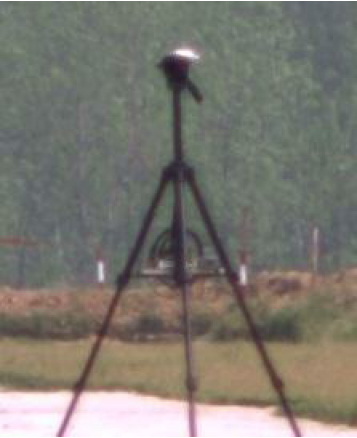
\includegraphics[width=0.4\textwidth]{figs/chp03_stereo/chp03_vision_16_dgps_calibration.pdf}	
	\caption{标定过程中,从左侧视觉系统中观察到的DGPS靶标}
	\label{fig:chp03_vision_16_dgps_calibration}
\end{figure}


相比于视觉系统的棋盘格标定方法,DGPS标定方法的优势是能够满足远距离标定需求。一般DGPS的设置点距离转台在$100\ m$以上,可以覆盖引导系统的末状态工作区域。而传统棋盘格由于制作尺寸受限,其标定范围一般在$5~10\ m$,该范围并不是转台经常工作的区域,其标定效果一般较差。

定义在下滑轨迹坐标系中任意一点的坐标为$(X_p, Y_p, Z_p)$,该点在引导坐标系的坐标系为$(X_c, Y_c, Z_c)$,因此需要求解这两个坐标系之间的转换矩阵
\begin{equation}
\left[ {\begin{array}{*{20}{c}}
	{{X_p}} \\ 
	{{Y_p}} \\ 
	{{Z_p}} 
	\end{array}} \right] = \mathcal{R}_c^p\left[ {\begin{array}{*{20}{c}}
	{{Z_{c}}} \\ 
	{{Y_{c}}} \\ 
	{{Z_{c}}} 
	\end{array}} \right] + T_c^p
\end{equation}
其中$\mathcal{R}_c^p$是$3\times3$旋转矩阵,$T_c^p$是$3\times1$平移矩阵。由于转换关系符合欧拉角定义,按照$\psi-\theta-\phi$的转换顺序,可以得到
\begin{equation}
\mathcal{R}_c^p = \begin{bmatrix}
\cos \theta \cos \psi                             & \cos\theta \sin\psi                               & -\sin\theta         \\
-\cos\phi \sin\psi + \sin\phi \sin\theta \cos\psi & \cos\phi \cos\psi + \sin\phi \sin\theta\sin\psi   & \sin\phi \cos\theta \\
\sin\phi \sin\psi + \cos\phi \sin\theta \cos\psi  & -\sin\phi \cos\psi + \cos\phi \sin\theta \sin\psi & \cos\phi \cos\theta
\end{bmatrix}
\end{equation}
上述转换矩阵中的欧拉角无法通过解析的方法求得,只能通过多次采集标定点数据最优迭代获得。因此,定义旋转矩阵和平移矩阵的分量为
\begin{equation}
\mathcal{R}_c^p = \begin{bmatrix}
r_{11} & r_{12} & r_{13}\\
r_{21} & r_{22} & r_{23}\\
r_{31} & r_{32} & r_{33}\\
\end{bmatrix}
\end{equation}

\begin{equation}
T_c^p=\left[ {\begin{array}{*{20}{c}}
	t_x \\ 
	t_y \\ 
	t_z 
	\end{array}} \right]
\end{equation}
当通过手动控制转台使得光心对准DGPS天线时,上述6个变量$(\phi\ \theta\ \psi\ t_x\ t_y\ t_z)$与转台角度俯仰角$\phi_l$和方位角$\psi_l$之间的关系为
\begin{equation}
\left\{ \begin{gathered}
\tan \phi_l = \frac{Y_p}{Z_p} \\
\tan \phi_l = \frac{X_p}{\sqrt{X_p^2+Z_p^2} }\\
\end{gathered}  \right.
\end{equation}

\begin{equation}
\left\{ \begin{gathered}
\tan \phi_l= \frac{r_{21}X_p + r_{22}Y_p + r_{23}Z_p + t_y}{r_{31}X_p + r_{32}Y_p + r_{33}Z_p + t_z} \\
\tan \psi_l= \frac{r_{11}X_p + r_{12}Y_p + r_{13}Z_p + t_y}{\sqrt{(r_{31}X_p + r_{32}Y_p + r_{33}Z_p + t_y)^2+(r_{21}X_p + r_{22}Y_p + r_{23}Z_p + t_y)^2} }\\
\end{gathered}  \right.
\end{equation}

二维转台DGPS方法标定的基本步骤如下:
\begin{compactenum}
	\item
	转台系统初始化,并归零。
	\item
	放置DGPS点在不同位置(不少于3组,一般为10组),并该点的DGPS数据和转台两个转动角度。
	\item
	将采集到的数据通过非线性最小二乘的方法求解得到上述6个标定参数。
\end{compactenum}
注意在标定过程中,尽可能保持DGPS横向($\mathbf{i}^{O,c}$轴向)移动的连续性,使得转台始终向一侧转动。由于转动机械机构的误差,转台出现连续向左和向右的运动,容易将误差放大。

\subsection{DGPS标定方法实验验证}
配置左右视觉单元的基线距离为$10\ m$,实验总共采集20组DGPS靶标数据,其中使用前10组数据进行参数的求解,使用后10组数据来验证上述标定方法的准确性。这些点选取的一般位于距离标定单元$100\ m$左右,尽可能覆盖转台方位角$-25\degree-25\degree$的范围,该标定区域的示意图如\ref{fig:chp03_vision_18_dgps_calibration_diagram}所示。其中一组标定数据集的系统标定参数如表\ref{label:dgps_calibration}所示。

\begin{figure}[htb]
	\centering
	\includegraphics[width=0.7\textwidth]{figs/chp03_stereo/chp03_vision_18_dgps_calibration_diagram.pdf}	
	\caption{DGPS标定过程中选定的20个标定点}
	\label{fig:chp03_vision_18_dgps_calibration_diagram}
\end{figure}

\begin{table}[htb]
	\centering
	\caption{DGPS标定方法得到的标定数据}
	\label{label:dgps_calibration}
	\begin{tabular}{ccccccc}
		\hline
		标定参数 & $\phi (\degree)$ & $\theta (\degree)$ & $\psi (\degree)$ & $t_x (m)$ & $t_y(m)$ & $t_z(m)$ \\ \hline
		实际数值 & 1.58             & -0.01              & 1.57             & -0.41     & 23.31   & -2.21    \\ \hline
	\end{tabular}
\end{table}

在得到上述标定参数后,通过后续10个测试数据来检验标定的精度。表\ref{label:DGPS_Pan_Tilit_Calibration_Error}是这是个测试DGPS点的真实值和解算值。其中,十组数据的方位角平均误差为$0.0141\degree$,俯仰角的平均误差为$-0.0319\degree$。每个标定点的误差曲线如图\ref{fig:chp03_vision_19_pan_tilt_ten_points_error}所示。

% /home/amax/Workspace/77.GOTURN/GOTURN/landing_original_folder/Landing_Data_1
\begin{table}[]
	\centering
	\caption{DGPS标定测试集误差}
	\label{label:DGPS_Pan_Tilit_Calibration_Error}
	\begin{tabular}{crrrr}
		\hline
		& \multicolumn{2}{c}{真实值$(\degree)$}                           & \multicolumn{2}{c}{标定值$(\degree)$}                           \\ \hline
		DGPS点编号 & \multicolumn{1}{c}{方位角} & \multicolumn{1}{c}{俯仰角} & \multicolumn{1}{c}{方位角} & \multicolumn{1}{c}{俯仰角} \\ \hline
		1       & 0.7843                  & -0.0836                 & 0.7730                  & -0.0691                 \\
		2       & 5.9854                  & 0.5722                  & 6.0372                  & 0.6129                  \\
		3       & 0.9065                  & 0.5722                  & 0.8573                  & 0.6404                  \\
		4       & -4.5582                 & 0.4757                 & -4.5237                 & 0.5322                  \\
		5       & -4.7832                 & 0.1350                  & -4.7748                 & 0.1343                  \\
		6       & 1.7294                  & 1.0094                  & 1.6185                  & 1.0921                  \\
		7       & 8.1520                  & 1.1122                  & 8.0970                  & 1.1053                  \\
		8       & -5.1689                 & 1.1701                  & -5.2517                 & 1.2527                  \\
		9       & 3.6645                  & 0.4307                  & 3.6734                  & 0.4075                  \\
		10      & -3.6388                 & 0.4565                  & -3.5739                 & 0.4614                  \\ \hline
	\end{tabular}
\end{table}


\begin{figure}[htb]
	\centering
	\includegraphics[width=\textwidth]{figs/chp03_stereo/chp03_vision_19_pan_tilt_ten_points_error.pdf}	
	\caption{DGPS标定测试集方位角和俯仰角误差曲线}
	\label{fig:chp03_vision_19_pan_tilt_ten_points_error}
\end{figure}

为了验证该标定方法的有效性,重复上述实验10次,得到的标定误差结果如表\ref{label:DGPS_10_Test_Results}所示。其中10组测试中两个角度的最大误差用粗体表示。通过实验可以看到,该方法的标定精读较高,能够满足坐标系转换需求。
\begin{table}[htb]
	\centering
	\caption{10组DGPS标定方法测试俯仰角和方位角误差}
	\label{label:DGPS_10_Test_Results}
	\begin{tabular}{crr}
		\hline
		实验组数 & \multicolumn{1}{c}{方位角误差平均值} & \multicolumn{1}{c}{俯仰角俯仰角误差平均值} \\ \hline
		1    & 0.0141                       & -0.0319                         \\
		2    & \textbf{-0.0211}             & 0.0221                          \\
		3    & 0.0085                       & -0.0322                \\
		4    & -0.0133                      & -0.0149                         \\
		5    & -0.0093                      & 0.0350                          \\
		6    & 0.0043                       & -0.0132                         \\
		7    & -0.0132                      & 0.0152                          \\
		8    & -0.0201                      & -0.0320                         \\
		9    & 0.0114                       & -0.0119                         \\
		10   & -0.0147                      & \textbf{0.0565}                          \\ \hline
	\end{tabular}
\end{table}

\section{本章小结}
本章通过误差分析和理论推导,设计基于立体视觉成像的短基线和长基线引导系统,实现对无人机相对位置的测量。并根据长基线立体视觉系统的特点,设计使用基于DGPS的标定方法。
